\documentclass[10pt, aspectratio=169]{beamer}
% Shared setup for every day of the course.
\usetheme[progressbar=frametitle, numbering=fraction, block=fill]{metropolis}
\usepackage[T1]{fontenc}
\usepackage[utf8]{inputenc}
\usepackage{lmodern}
\usepackage{amsmath, amssymb, bm, booktabs, graphicx, xcolor, colortbl}
\usepackage{tikz}
\usetikzlibrary{arrows.meta, positioning, calc, shapes.geometric, decorations.pathreplacing}

\graphicspath{{figures/}}

% --- colours -------------------------------------------------------------------------------------
\definecolor{accent}{HTML}{C0392B}
\definecolor{cool}{HTML}{2E6DB4}
\definecolor{muted}{HTML}{7A7A7A}
\definecolor{good}{HTML}{2E8B57}
\setbeamercolor{alerted text}{fg=accent}
\setbeamercolor{example text}{fg=cool}

% --- notation (follows the thesis' notation chapter) ---------------------------------------------
\newcommand{\given}{\,|\,}
\newcommand{\E}{\mathbb{E}}
\newcommand{\KL}[2]{D_{\mathrm{KL}}\!\left[#1\,\middle\|\,#2\right]}
\newcommand{\N}{\mathcal{N}}
\newcommand{\Hess}{\mathcal{H}}
\newcommand{\nats}{\,\text{nats}}
\DeclareMathOperator*{\argmin}{arg\,min}

% --- course devices ------------------------------------------------------------------------------
% \src{...}: where a claim or number comes from (thesis file and line, or a post-thesis note).
\newcommand{\src}[1]{\par\vfill\hfill{\scriptsize\color{muted}source: #1}}
% \wip: marks a post-thesis result.
\newcommand{\wip}{{\scriptsize\color{white}\colorbox{accent}{\,work in progress\,}}}
% \lesson{...}: the one sentence a frame exists to say.
% one full-width band, no empty title bar above it
\newcommand{\lesson}[1]{\par\vspace{0pt plus 1filll}\begin{beamercolorbox}[wd=\linewidth, sep=0.45em, center]{block body alerted}#1\end{beamercolorbox}}
% space under every frame title, so content never starts flush against the title bar
\addtobeamertemplate{frametitle}{}{\vspace*{0.8em minus 0.8em}}
% a measurement story
\newenvironment{measured}[1]{\begin{exampleblock}{Measured: #1}}{\end{exampleblock}}

\institute{Montevideo, 30 November -- 4 December 2026}

% \cyclemap{n}: the course's five-stage cycle, stage n highlighted (1 room ... 5 memory).
\newcommand{\cyclemap}[1]{%
  \begin{tikzpicture}[
      st/.style={draw=muted, thick, rounded corners=3pt, fill=white, align=center,
                 minimum width=2.5cm, minimum height=0.8cm, font=\scriptsize, text=muted},
      on/.style={draw=accent, very thick, fill=accent!10, text=black, font=\scriptsize\bfseries},
      arr/.style={-{Stealth[length=2mm]}, thick, color=muted},
      s1/.style={}, s2/.style={}, s3/.style={}, s4/.style={}, s5/.style={}, s#1/.style={on}]
    \node[st, s1] (c1) at (90:1.9)   {estimate the room};
    \node[st, s2] (c2) at (18:2.6)   {localise; learn\\the body};
    \node[st, s3] (c3) at (-54:2.2)  {concepts fill\\the room};
    \node[st, s4] (c4) at (-126:2.2) {cross the door};
    \node[st, s5] (c5) at (162:2.6)  {new room;\\memory};
    \draw[arr] (c1) to[bend left=15] (c2); \draw[arr] (c2) to[bend left=15] (c3);
    \draw[arr] (c3) to[bend left=15] (c4); \draw[arr] (c4) to[bend left=15] (c5);
    \draw[arr] (c5) to[bend left=15] (c1);
  \end{tikzpicture}}


\title{A robot that acts to know}
\subtitle{Day 5 --- Talking to the robot, and what comes next}
\date{Friday 4 December}

\tikzset{box4/.style={draw, rounded corners=3pt, thick, align=center, font=\footnotesize, minimum height=0.8cm},
         arr4/.style={-{Stealth[length=2.5mm]}, thick},
         lab4/.style={font=\scriptsize},
         c/.style={draw=#1, thick, rounded corners=3pt, fill=#1!8, align=center, font=\scriptsize, text width=3.7cm, minimum height=1.25cm, inner sep=3pt}}
\tikzset{bx/.style={draw, rounded corners=3pt, thick, align=center, font=\footnotesize,
                    minimum height=0.8cm, inner sep=3pt},
         lab/.style={font=\scriptsize},
         arr/.style={-{Stealth}, thick},
         obj/.style={draw, circle, thick, inner sep=0pt, minimum size=0.55cm, font=\scriptsize},
         flow/.style={-{Stealth[length=2.5mm]}, thick},
         mtag/.style={draw, thick, rounded corners=2pt, font=\scriptsize, inner sep=3pt, fill=white, align=center, minimum height=0.85cm, text width=#1, anchor=north},
         mtag/.default=2.6cm,
         dimcard/.style={draw=#1, thick, rounded corners=4pt, fill=#1!12, minimum width=4.5cm, minimum height=1.42cm, align=center, font=\footnotesize, inner sep=3pt}}

% \chairside{x,y}{seat width}{seat height}{back height}{style}: a chair seen from the side.
\newcommand{\chairside}[5]{
  \draw[#5, line join=round, line cap=round] ($(#1)+(-0.14,#3+#4)$) -- ($(#1)+(0,#3)$) -- ($(#1)+(#2,#3)$) -- ($(#1)+(#2+0.08,0)$);
  \draw[#5, line cap=round] ($(#1)+(0,#3)$) -- ($(#1)+(-0.1,0)$);
}


\begin{document}

\maketitle

\begin{frame}{Today: the person talks to the robot, and the robot to itself}
  \centering
  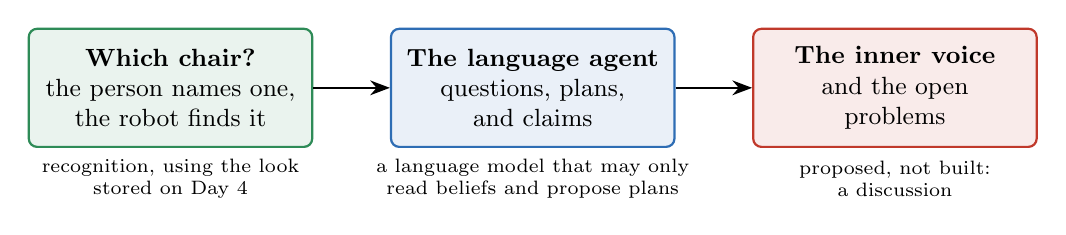
\begin{tikzpicture}[s/.style={box4, minimum width=3.6cm, minimum height=1.5cm, font=\small}]
    \node[s, draw=good, fill=good!10] (a) at (0,0) {\textbf{Which chair?}\\the person names one,\\the robot finds it};
    \node[s, draw=cool, fill=cool!10] (l) at (4.6,0) {\textbf{The language agent}\\questions, plans,\\and claims};
    \node[s, draw=accent, fill=accent!10] (v) at (9.2,0) {\textbf{The inner voice}\\and the open\\problems};
    \draw[arr4] (a) -- (l); \draw[arr4] (l) -- (v);
    \node[lab4, align=center] at (0,-1.15) {recognition, using the look\\stored on Day 4};
    \node[lab4, align=center] at (4.6,-1.15) {a language model that may only\\read beliefs and propose plans};
    \node[lab4, align=center] at (9.2,-1.15) {proposed, not built:\\a discussion};
  \end{tikzpicture}

  \vspace{1em}
  \small The beliefs are the ones built this week. Language adds no new belief of its own.
  \lesson{Language reads and changes the same beliefs the agents built this week.}
\end{frame}

% =================================================================================================
\section{Which chair do you mean?}
% =================================================================================================


\begin{frame}{A second sight is a comparison, and ``new'' is on the list}
  \begin{columns}[c]
    \begin{column}{0.44\textwidth}
      \centering
      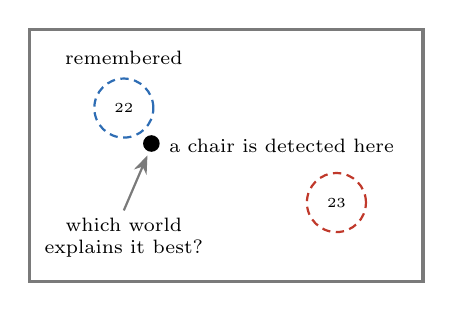
\begin{tikzpicture}
        \draw[very thick, muted] (0,0) rectangle (5,3.2);
        \node[draw=cool, densely dashed, thick, circle, minimum size=0.75cm, font=\tiny] (a) at (1.2,2.2) {22};
        \node[draw=accent, densely dashed, thick, circle, minimum size=0.75cm, font=\tiny] (b) at (3.9,1.0) {23};
        \node[lab, above=1pt] at (a.north) {remembered};
        \fill[black] (1.55,1.75) circle (3pt);
        \node[lab, right] at (1.65,1.72) {a chair is detected here};
        \draw[-{Stealth}, muted, thick] (1.2,0.9) -- (1.5,1.6);
        \node[lab, align=center] at (1.2,0.55) {which world\\explains it best?};
      \end{tikzpicture}\\[0.4em]
      \footnotesize
      \begin{tabular}{@{}l l@{}}
        is it chair 22? & $\ln p(x\,|\,22) + r_{22}$\\
        is it chair 23? & $\ln p(x\,|\,23) + r_{23}$\\
        is it \textbf{new}? & $\ln (1/A)$\\
      \end{tabular}
    \end{column}
    \begin{column}{0.53\textwidth}
      \small
      Where it is: the chair stayed, or it was moved with probability $\pi$ and could be anywhere:
      \[ p(x\,|\,k) = (1-\pi)\,\N(x;\mu_k,\Sigma) + \pi/A . \]
      What it looks like: $r_k$, the nats by which this chair's views explain the view better than
      the class does.\\[0.5em]
      Long-term memory only offers. The chair agent decides, the winner must beat ``new'', and a tie
      goes to ``new''.\\[0.5em]
      \alert{On position alone a moved chair cannot win: $\pi/A<1/A$.}
    \end{column}
  \end{columns}
\end{frame}

\begin{frame}{Second sight: what the toy says, what the robot does \wip}
  \begin{columns}[T]
    \begin{column}{0.5\textwidth}
      \footnotesize
      \textbf{Toy, \% identified correctly}\\[0.3em]
      \begin{tabular}{@{}l r r r@{}}
        \toprule
         & position & + look & + look,\\
         & & & same model \\
        \midrule
        chair stayed & 98 & 100 & 99 \\
        chair moved & 6 & 100 & \alert{33} \\
        new chair & 81 & 100 & \alert{0} \\
        \bottomrule
      \end{tabular}

      \vspace{0.6em}
      With views twice as noisy as the model assumes, the look keeps only \alert{42\%} of the chairs
      that never moved. Position alone kept 98\%.
    \end{column}
    \begin{column}{0.47\textwidth}
      \begin{measured}{chairs, in simulated tours}\footnotesize
        Position only, no appearance term. Back in the room, chairs return under their old identity
        (p $.92$--$.98$), also from a previous start of the system.
      \end{measured}
      \footnotesize
      \begin{itemize}
        \item The chair is absent for about 35 s after the return, until it is detected again.
        \item A \alert{moved} chair is not established: replaying the atlas offline, 15 of 53 right.
        \item Other classes: merged, never run. Renaming and learned permanence: designed only.
      \end{itemize}
    \end{column}
  \end{columns}
\end{frame}

% =================================================================================================
\section{\texorpdfstring{Talking to the robot\\[0.4em]{\normalsize\mdseries\color{muted} language reads and changes the same beliefs}}{Talking to the robot}}
% =================================================================================================


\begin{frame}{The language agent: a language model that acts only through tools}
  \centering
  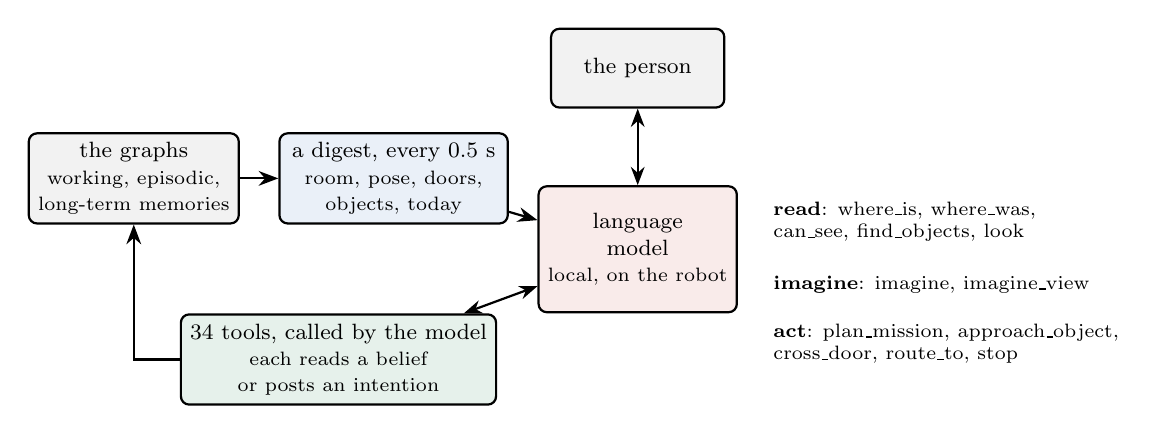
\begin{tikzpicture}[s/.style={box4, minimum height=1.0cm}]
    \node[s, fill=muted!10, minimum width=2.6cm] (g) at (0,0.9) {the graphs\\\scriptsize working, episodic,\\\scriptsize long-term memories};
    \node[s, fill=cool!10, minimum width=2.9cm] (d) at (3.3,0.9) {a digest, every 0.5 s\\\scriptsize room, pose, doors,\\\scriptsize objects, today};
    \node[s, fill=accent!10, minimum width=2.4cm, minimum height=1.6cm] (m) at (6.4,0) {language\\model\\{\scriptsize local, on the robot}};
    \node[s, fill=muted!10, minimum width=2.2cm] (p) at (6.4,2.3) {the person};
    \node[s, fill=good!12, minimum width=2.7cm] (t) at (2.6,-1.4) {34 tools, called by the model\\\scriptsize each reads a belief\\\scriptsize or posts an intention};
    \draw[arr4] (g) -- (d); \draw[arr4] (d) -- (m);
    \draw[arr4, Stealth-Stealth] (p) -- (m);
    \draw[arr4, Stealth-Stealth] (m) -- (t);
    \draw[arr4] (t) -| (g);
    \node[lab4, align=left, anchor=west] at (8.0,0.35) {\textbf{read}: where\_is, where\_was,\\can\_see, find\_objects, look};
    \node[lab4, align=left, anchor=west] at (8.0,-0.45) {\textbf{imagine}: imagine, imagine\_view};
    \node[lab4, align=left, anchor=west] at (8.0,-1.2) {\textbf{act}: plan\_mission, approach\_object,\\cross\_door, route\_to, stop};
  \end{tikzpicture}

  \vspace{0.6em}
  \small The model sees a text digest of the graph, never the graph itself. Notes on missions, doors and
  exploring are loaded only when the model asks for them.
  \lesson{The model answers from the digest and acts through tools; each tool touches one belief.}
\end{frame}

\begin{frame}[t]{The language model proposes; the controller acts}
  \centering
  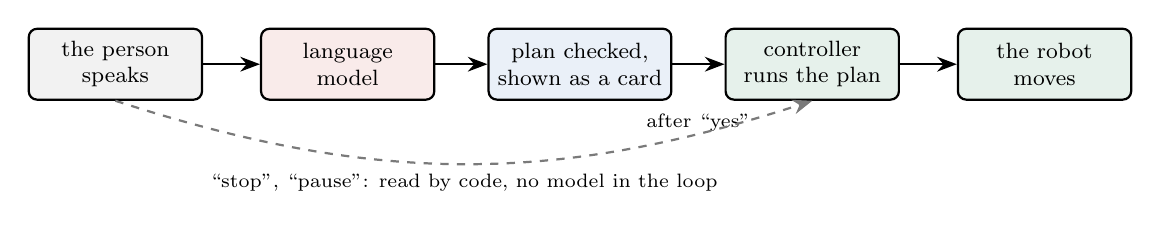
\begin{tikzpicture}[s/.style={box4, minimum width=2.2cm, minimum height=0.9cm}]
    \node[s, fill=muted!10] (p) at (0,0) {the person\\speaks};
    \node[s, fill=accent!10] (l) at (2.95,0) {language\\model};
    \node[s, fill=cool!10] (c) at (5.9,0) {plan checked,\\shown as a card};
    \node[s, fill=good!12] (k) at (8.85,0) {controller\\runs the plan};
    \node[s, fill=good!12] (r) at (11.8,0) {the robot\\moves};
    \draw[arr4] (p) -- (l);
    \draw[arr4] (l) -- (c);
    \draw[arr4] (c) -- node[below=0.5cm, lab4] {after ``yes''} (k);
    \draw[arr4] (k) -- (r);
    \draw[arr4, muted, dashed] (p.south) to[bend right=18] node[below, lab4, text=black] {``stop'', ``pause'': read by code, no model in the loop} (k.south);
  \end{tikzpicture}

  \vspace{0.3em}
  \begin{columns}[T]
    \begin{column}{0.53\textwidth}
      \footnotesize
{\ttfamily\scriptsize\raggedright
      mission "go to room\_3 and tell me the colour\\
      \hspace*{4.4em}of every chair on the way"\\
      \hspace*{1em}watch seen(chair) continue each=c\\
      \hspace*{2em}report "the colour of \$c"\\
      \hspace*{1em}cross door\_22 expect=room\_3 retry=2\par}
    \end{column}
    \begin{column}{0.43\textwidth}
      \small
      The plan is written in a small mission language: steps, conditions such as
      \texttt{door\_open(door\_1)<0.5}, and watches on what is seen.\\[0.4em]
      A condition reads a belief: $P(\text{open})$ is the door agent's.
    \end{column}
  \end{columns}
  \lesson{The language model writes plans; it never drives the robot.}
\end{frame}

\begin{frame}[t]{A question is a query on a belief the robot already holds}
  \centering\small
  \renewcommand{\arraystretch}{1.25}
  \begin{tabular}{@{}p{3.9cm} p{3.6cm} p{5.3cm}@{}}
    \toprule
    the person asks & who holds the belief & the answer \\
    \midrule
    ``Where is my chair?'' & long-term object memory & its last seen room and pose, copied, not rephrased \\
    ``Is door\_1 open?'' & the door agent & $P(\text{open})$ from the leaf angle it observes \\
    ``Can you see the fridge from the door?'' & every concept agent publishes how it detects & $P(\text{see}\given\mathbf v)$ \\
    \bottomrule
  \end{tabular}

  \vspace{-0.3em}
  \[
    P(\text{see}\given\mathbf v) \;=\; P(\text{notice}\given\mathbf v)\;\cdot\;P(\text{recognise}\given\mathbf v)
  \]
  \raggedright\small
  $\mathbf v$: where the robot would stand. \emph{Notice}: enough of the object is in view past walls and
  doors. \emph{Recognise}: the detector names it at that distance. The same $P(\text{detect}\given\mathbf v)$
  that priced a view yesterday.
  \lesson{The language model chooses which belief to ask; the number comes from the belief.}
\end{frame}

\begin{frame}[t]{Imagining: the same model, run on a changed copy of the world}
  \centering
  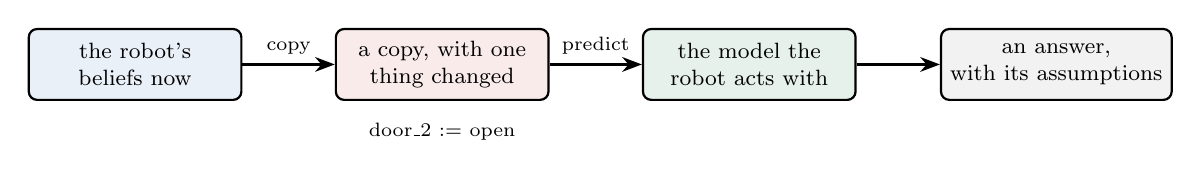
\begin{tikzpicture}[s/.style={box4, minimum width=2.7cm, minimum height=0.9cm}]
    \node[s, fill=cool!10] (w) at (0,0) {the robot's\\beliefs now};
    \node[s, fill=accent!10] (x) at (3.9,0) {a copy, with one\\thing changed};
    \node[s, fill=good!12] (m) at (7.8,0) {the model the\\robot acts with};
    \node[s, fill=muted!10] (a) at (11.7,0) {an answer,\\with its assumptions};
    \draw[arr4] (w) -- node[above, lab4] {copy} (x);
    \draw[arr4] (x) -- node[above, lab4] {predict} (m);
    \draw[arr4] (m) -- (a);
    \node[lab4, below=0.15cm of x, align=center] {door\_2 := open};
  \end{tikzpicture}

  \vspace{0.8em}
  \small
  \renewcommand{\arraystretch}{1.4}
  \begin{tabular}{@{}p{5.4cm} p{7.0cm}@{}}
    \toprule
    ``Would I fit through door\_2?'' & the controller's own fitting model and the robot's footprint \\
    ``Would I see the fridge if door\_2 were open?'' & $P(\text{see}\given\mathbf v)$ on the changed copy \\
    ``Would I get through door\_1?'' & the robot's past crossings of that door, counted \\
    \bottomrule
  \end{tabular}
  \lesson{To imagine is to predict observations under a change: what expected free energy needs.}
\end{frame}

\begin{frame}[t]{Every claim must come from a tool that read a belief}
  \begin{columns}[T]
    \begin{column}{0.48\textwidth}
      \textbf{The person's words become a belief only after a check}
      \vspace{0.4em}

      \centering
      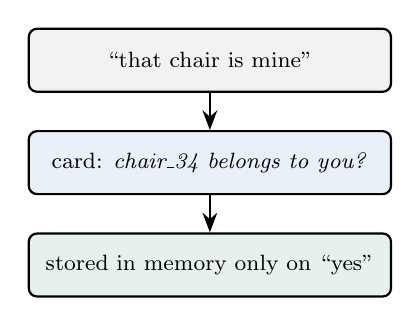
\begin{tikzpicture}[s/.style={box4, minimum width=4.6cm}]
        \node[s, fill=muted!10] (a) at (0,0) {``that chair is mine''};
        \node[s, fill=cool!10] (b) at (0,-1.3) {card: \emph{chair\_34 belongs to you?}};
        \node[s, fill=good!12] (c) at (0,-2.6) {stored in memory only on ``yes''};
        \draw[arr4] (a) -- (b); \draw[arr4] (b) -- (c);
      \end{tikzpicture}
    \end{column}
    \begin{column}{0.48\textwidth}
      \textbf{The model's words, when no tool ran}
      \vspace{0.4em}

      \centering
      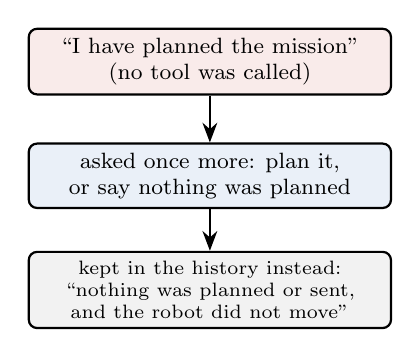
\begin{tikzpicture}[s/.style={box4, minimum width=4.6cm}]
        \node[s, fill=accent!10] (a) at (0,0) {``I have planned the mission''\\(no tool was called)};
        \node[s, fill=cool!10] (b) at (0,-1.45) {asked once more: plan it,\\or say nothing was planned};
        \node[s, fill=muted!10, font=\scriptsize] (c) at (0,-2.9) {kept in the history instead:\\``nothing was planned or sent,\\and the robot did not move''};
        \draw[arr4] (a) -- (b); \draw[arr4] (b) -- (c);
      \end{tikzpicture}
    \end{column}
  \end{columns}

  \vspace{0.5em}
  \small If the false sentence stayed in the history, the model would copy it the next time.
  \lesson{The language model is not the robot's belief: it may only report what a tool returned.}
\end{frame}

% =================================================================================================
\section{The inner voice, and open directions}
% =================================================================================================


\begin{frame}[t]{From speech between people to speech inside \hfill\wip}
  \centering
  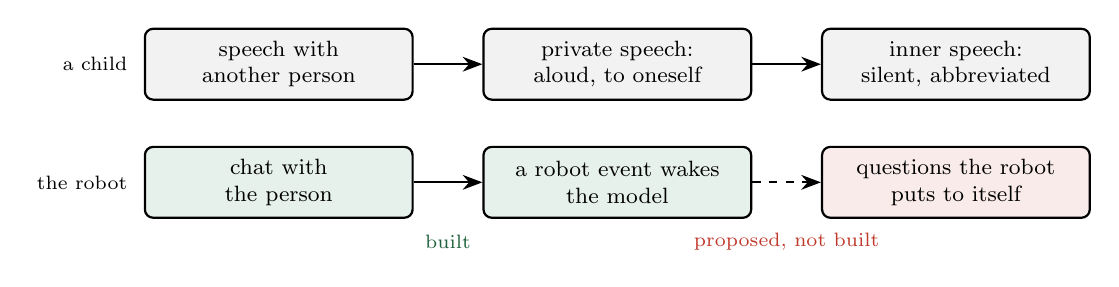
\begin{tikzpicture}[s/.style={box4, minimum width=3.4cm, minimum height=0.9cm}]
    \node[lab4, anchor=east] at (-1.8,0) {a child};
    \node[s, fill=muted!10] (a) at (0,0) {speech with\\another person};
    \node[s, fill=muted!10] (b) at (4.3,0) {private speech:\\aloud, to oneself};
    \node[s, fill=muted!10] (c) at (8.6,0) {inner speech:\\silent, abbreviated};
    \draw[arr4] (a) -- (b); \draw[arr4] (b) -- (c);
    \node[lab4, anchor=east] at (-1.8,-1.5) {the robot};
    \node[s, fill=good!12] (d) at (0,-1.5) {chat with\\the person};
    \node[s, fill=good!12] (e) at (4.3,-1.5) {a robot event wakes\\the model};
    \node[s, fill=accent!10] (f) at (8.6,-1.5) {questions the robot\\puts to itself};
    \draw[arr4] (d) -- (e); \draw[arr4, dashed] (e) -- (f);
    \node[lab4] at (2.15,-2.25) {\color{good!70!black}built};
    \node[lab4] at (6.45,-2.25) {\color{accent}proposed, not built};
  \end{tikzpicture}

  \vspace{0.2em}
  \raggedright\small
  Vygotsky: a function appears first between people, then inside the individual. Children talk aloud
  to themselves more when the task is harder.\\[0.3em]
  A wake today: during a mission, a robot event goes to the model, which may look, query, stop or
  propose, and may not act.
  \lesson{The robot's inner voice would be the chat, turned inward on its own surprises.}
\end{frame}

\begin{frame}[t]{An inner question is a small active-inference loop \hfill\wip}
  \centering
  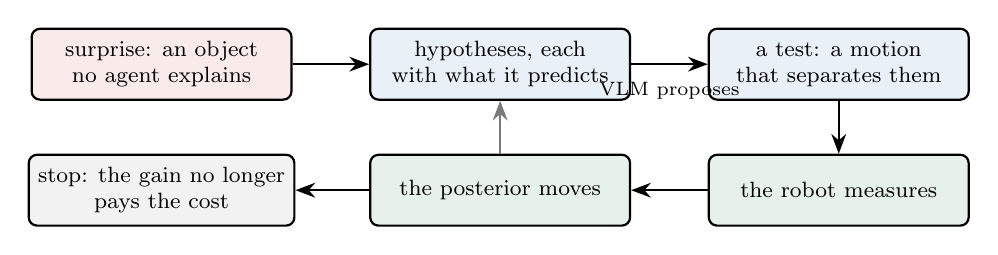
\begin{tikzpicture}[s/.style={box4, minimum width=3.3cm, minimum height=0.9cm}]
    \node[s, fill=accent!10] (q) at (0,0) {surprise: an object\\no agent explains};
    \node[s, fill=cool!10] (h) at (4.3,0) {hypotheses, each\\with what it predicts};
    \node[s, fill=cool!10] (t) at (8.6,0) {a test: a motion\\that separates them};
    \node[s, fill=good!12] (m) at (8.6,-1.6) {the robot measures};
    \node[s, fill=good!12] (p) at (4.3,-1.6) {the posterior moves};
    \node[s, fill=muted!10] (e) at (0,-1.6) {stop: the gain no longer\\pays the cost};
    \draw[arr4] (q) -- (h); \draw[arr4] (h) -- node[below=0.1cm, lab4] {VLM proposes} (t);
    \draw[arr4] (t) -- (m); \draw[arr4] (m) -- (p); \draw[arr4] (p) -- (e);
    \draw[arr4, muted] (p) -- (h);
  \end{tikzpicture}

  \vspace{0.2em}
  \raggedright\small
  \textbf{Illustrative, not a run:} bag, robot vacuum or moved chair? The vision-language model
  proposes ``approach to 1 m: a vacuum is under 0.15 m tall and moves''. The robot measures 0.12 m and
  sees it move.\\[0.3em]
  The model only sets what each hypothesis predicts. \alert{Only the robot's own measurement moves
  the posterior.}
  \lesson{Talking to oneself is choosing the next look by expected information gain.}
\end{frame}

\begin{frame}{What is measured, and what is not}
  \begin{columns}[T]
    \begin{column}{0.5\textwidth}
      \begin{measured}{a local model writes the plans}
        \small
        On a robot-mounted computer, a 26-billion-parameter open model wrote correct missions
        for 66 of 72 requests (24 requests, 3 runs each), in under a second.
      \end{measured}
      \small
      In one simulated run a watch reacted while the robot crossed a door, and a ``stop'' watch ended
      an exploration at a new chair.
    \end{column}
    \begin{column}{0.46\textwidth}
      \small
      \textbf{Not established:}
      \begin{itemize}
        \item the inner voice: designed, not built, nothing run;
        \item the prediction that inner questions fall with practice, as private speech does
              (a cache would show it too);
        \item phrase lists catch false claims in English and Spanish only.
      \end{itemize}
    \end{column}
  \end{columns}
\end{frame}

\begin{frame}{Open directions: what this week left unbuilt}
  \centering
  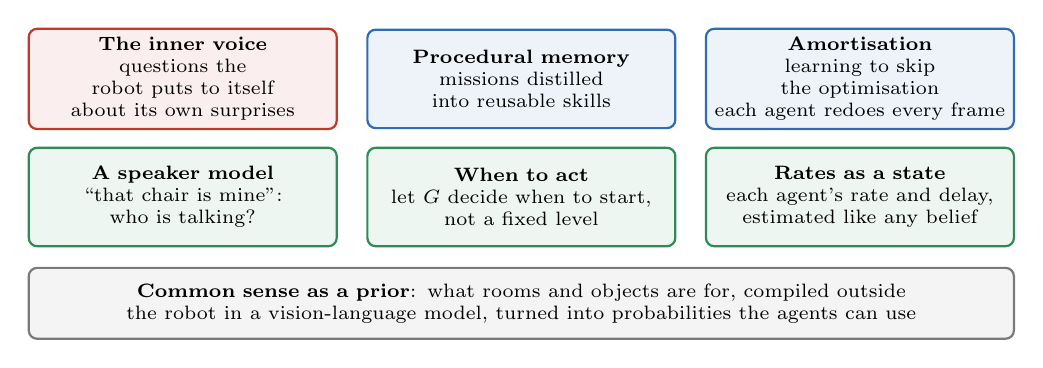
\begin{tikzpicture}
    \node[c=accent] at (0,1.5)   {\textbf{The inner voice}\\questions the robot puts to itself\\about its own surprises};
    \node[c=cool]   at (4.3,1.5) {\textbf{Procedural memory}\\missions distilled\\into reusable skills};
    \node[c=cool]   at (8.6,1.5) {\textbf{Amortisation}\\learning to skip the optimisation\\each agent redoes every frame};
    \node[c=good]   at (0,0)     {\textbf{A speaker model}\\``that chair is mine'':\\who is talking?};
    \node[c=good]   at (4.3,0)   {\textbf{When to act}\\let $G$ decide when to start,\\not a fixed level};
    \node[c=good]   at (8.6,0)   {\textbf{Rates as a state}\\each agent's rate and delay,\\estimated like any belief};
    \node[c=muted, text width=12.3cm, minimum height=0.9cm] at (4.3,-1.35) {\textbf{Common sense as a prior}: what rooms and objects are for,
      compiled outside the robot in a vision-language model, turned into probabilities the agents can use};
  \end{tikzpicture}

  \vspace{0.6em}
  \small For discussion: which would you build first, and what would it change in the robot?
  \lesson{Each open problem is a belief nobody holds yet, or a choice still made by a rule.}
\end{frame}

% =================================================================================================
\section{Lab}
% =================================================================================================


\begin{frame}{Lab 5: which chair, and a language agent that cannot lie}
  \texttt{labs/day5.ipynb}, about two hours.
  \begin{columns}[T]
    \begin{column}{0.46\textwidth}
      \small
      \textbf{A. Second sight}
      \begin{itemize}
        \item three remembered chairs and ``new'';
        \item position against look; one model of chair;
        \item a view from the other side.
      \end{itemize}
    \end{column}
    \begin{column}{0.5\textwidth}
      \small
      \textbf{B. A toy language agent}
      \begin{itemize}
        \item write tools that read beliefs on the toy graph;
        \item a scripted model calls them; check every claim against a tool result;
        \item plan a mission with a condition on $P(\text{open})$;
        \item optional: replace the script by a local model.
      \end{itemize}
    \end{column}
  \end{columns}
  \vspace{0.6em}
  \small Short of time: A, then B up to the claim check.
  \lesson{The rule ``say only what a tool returned'' becomes a test you can run.}
\end{frame}

\begin{frame}{The last result of the week}
  \centering
  \vspace{1em}
  \raggedright
  \alert{The robot acts to make its beliefs better, and language is one more way to read and change
  those beliefs.} Whatever it says, it can show where it came from: a belief, the model that built it,
  and the look that paid for it.
\end{frame}

\end{document}
